%  Created by Branden Stone on 2015-01-15.
%  Copyright (c) 2015 Branden Stone. All rights reserved.
%--------------------------------------------------------
\documentclass{article}


%---------------------------
% Packages
%---------------------------
\usepackage{amssymb, amsmath, latexsym, amsfonts, amsthm, mathrsfs} % Standard packages that are nice to have.
\usepackage{amsrefs} % Allows for easy referencing and citations.
\usepackage{verbatim} % Needed for \begin{comment} \end{comment}.
\usepackage[text={6in,9in},centering]{geometry} % Defines the dimensions of the text body.
\usepackage[colorlinks=true]{hyperref} % Allows for use of hyperlinks.
%\usepackage[doublespacing]{setspace} % Makes the document double spaced.
\usepackage[pdftex]{graphicx} % Allows for \includegraphics
\usepackage{enumerate} % Allows for easy modification of lists

\renewcommand{\arraystretch}{1.5}

%----------------------------
% Title and Author
%----------------------------

\title{Math 390 Homework 8}
\author{Due Friday, April 22}
\date{}


%----------------------------
% Main Document Body
%----------------------------

\begin{document}


%-------------------------------------------------------------
% Front Matter: This is where you can add a table of contents,
% preface, list of figures, ETC. for this template we will 
% only create a title and author name with `\maketitle'
%-------------------------------------------------------------

\maketitle

\setlength{\parindent}{0em} % Sets indentation of new paragraph
\setlength{\parskip}{1em} % Sets space between paragraphs

%-------------------------------------------------------------
% Document Body: Essentially this is where you place the 
% content of your document. To use this template, just delete
% all of the text between here and the Bibliography Section.
% Then type whatever you desire.
%-------------------------------------------------------------


Solutions should be written \LaTeX\ or Markdown and converted to a PDF. You are encouraged to work with others
on the assignment, but you should write up your own solutions independently. This means no copy pasting. You should
reference all of your sources, including your collaborators. 

\begin{enumerate}

\item For each of the following graphs, compute the chromatic index $\chi'(G)$ of the graph, and show an edge-coloring that uses the minimum number of colors.
\begin{center}
	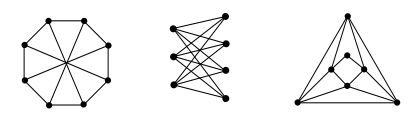
\includegraphics[width=.7\textwidth]{pic1.png}
\end{center}

\item \begin{enumerate}
	\item Prove that the chromatic polynomial of $K_{2,s}$ is 
		\[
			k(k-1)^s + k(k-1)(k-2)^s.
		\]

	\item Prove that the chromatic polynomial of $C_n$ is 
		\[
			(k-1)^n + (-1)^n(k-1).
		\]	
\end{enumerate}

\item  For each of the following bipartite graphs determine whether the graph has a complete matching. Justify your answers.
\begin{center}
	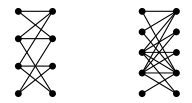
\includegraphics[width=.3\textwidth]{pic2.png}
\end{center}


\item Tom goes for a run every morning. When he leaves his house for his run he is equally likely to go out either the front or the back door; and similarly, when he returns he is equally likely to go to either the front or back door. He owns 5 pairs of running shoes, which he takes off after the run at whichever door he happens to be. If there are no shoes at the door from which he leaves to go running he runs barefooted.

\begin{enumerate}
	\item Model this situation with a Markov chain. (You will need to decide what the states of the Markov chain are.) Write down the transition matrix and associated digraph.

	\item Is this Markov chain ergodic? Explain your answer.

	\item In the long run, what proportion of days does he run barefooted? Justify your answer.
\end{enumerate}






\end{enumerate}




\end{document}